% ABLS - term-long paper
% Christopher Wood

\documentclass{sig-alternate}

\usepackage{url}
\usepackage{color}
\usepackage{enumerate}
\usepackage{balance}
\usepackage{verbatim}
\usepackage{enumitem}
\usepackage[table]{xcolor}
\usepackage{multicol,multirow}
\usepackage{subfig}
\usepackage{dcolumn}
\usepackage{palatino}
\usepackage{bbm}
\usepackage{url}
\usepackage{verbatim}
\usepackage{algorithm}
\usepackage[noend]{algorithmic}
\usepackage{fancybox, fancyvrb}
\usepackage{listings}
\usepackage{amsmath}
\usepackage{array}
\usepackage{mathtools}

\newenvironment{definition}[1][Definition]{\begin{trivlist}
\item[\hskip \labelsep {\bfseries #1}]}{\end{trivlist}}

\permission{}
\CopyrightYear{2012}
%\crdata{0-00000-00-0/00/00}
\begin{document}

\title{ABLS: Working Towards Attribute-Based Log Security and Automated Auditing in the Cloud}
\numberofauthors{1}
\author{
\alignauthor{
Christopher A. Wood \\
Department of Computer Science \\
{\tt caw4567@rit.edu}
}}
\date{\today}
\maketitle
\begin{abstract}
User-based non-repudiation is an increasingly important property of cloud-based applications. It provides irrefutable 
evidence that ties system behavior to specific users, thus enabling strict enforcement of organizational security policies. 
System logs are typically used as the basis for this property. Thus, the effectiveness of system audits based on log files 
reduces to the problem of maintaining the integrity and confidentiality of log files without sacrificing the usefulness
of the data in these log files. In an ideal setting, automated audits would be possible on encrypted log data that defines
audit trails. Furthermore, since useful log messages may contain sensitive information, access control for log 
data should be implemented so as to restrict access to only those parties that need to view it (i.e. generating users,
colleagues of generating users, auditors, system administrators, etc). ABAC has been a common technique used to
satisfy this requirement. %with the expense of role explosion. 

In this paper we address all of the aforementioned issues with ABLS, an attribute-based logging system designed
to support automates audits of encrypted audit trails (log data) based on user-defined security policies. Access to
sensitive log information is enforced using ciphertext-policy attribute-based encryption (CP-ABE) with a minimal number
of log-related roles, and thus a small number of attributes, to avoid the problem of increasing encryption computational
complexity with attribute explosion. We present the preliminary design of ABLS and discuss how audit trails are 
constructed, automated audit tasks are defined and specified, and how the system may be used in practical applications.
\end{abstract}

\section{Introduction}
User-based non-repudiation is a system security property that provides indisputable evidence linking
specific actions to individual users (or entities) that trigger such actions. Cryptographically speaking, 
non-repudiation requires that the integrity and 
origin of all data should be provable. In essence, this enables system audits to be conducted that can
identify data misuse, and thus, potential security policy violations, by comparing the contextual information 
of system events (e.g. source user, time of the event, etc) with all entities authorized to invoke such events. 
Therefore, treating non-repudiation as a required system quality attribute in the architecture is likely to 
become a common trend in the commercial, government, and even more specifically, the health-care domain.

System audits typically use log files to determine the ``who, what, when, and how'' of events that took 
place during the system's lifetime. In order to provide accurate information for non-repudiation purposes,
it is often necessary to place some amount user-sensitive data in these log files that can be used
to trace data back to its origin. As such, logs of events generated by a client that is being served must
maintain data confidentiality and integrity should the system be compromised. Historical approaches
to the problem of log security are based on tamper-resistant hardware and maintaining continuous 
secure communication channels between a log aggregator and end user \cite{Schneier1999-Secure}. 
However, such solutions are not applicable in the context of cloud-based applications. 

Recent approaches have relied on combinations of encryption and signature techniques \cite{Ma2008-FssAgg}. 
Symmetric-key and public-key encryption (and verification) of log entries are very common confidentiality techniques 
proposed in the literature. Unfortunately, these schemes are becoming less useful in cloud-based applications.
There is a need for robust access control mechanisms that enable dynamic user addition and revocation
with minimal overhead. In other words, continuously re-encrypting a subset of the log database should be avoided. 
Both symmetric- and public-key cryptosystems suffer in that access policies must be tied directly to keys used for
encryption and decryption. If the access policy for a set of log messages needs to be changed, then both the keys used to
encrypt and decrypt such log entries will need to be regenerated and distributed, and the entries must also
be re-encrypted. Both of these tasks can be very expensive. 

In addition, symmetric-key cryptosystems require keys to be shared among users who need access to the 
same set of logs. This requires a secure and comprehensive key management and distribution scheme and
supporting policy. In a similar vein, public-key cryptosystems (e.g. RSA and ElGamal) suffer 
from the extra data transfer and storage requirements for large cryptographic keys and certificates. There 
may be insufficient resources to maintain a public-key infrastructure (PKI) for managing keys and digital 
certificates for all users. 

In terms of log file integrity, aggregate signature schemes that support forward secrecy through the use of 
symmetric- and public-key cryptosystems are also becoming outdated \cite{Yavuz2009-BAF}. 
Symmetric-key schemes may promote high computational efficiency for signature generation, but they 
do not directly support public verifiability for administrators and auditors. This means that robust key 
distribution schemes or the introduction of a trusted third party (TTP) are needed to ensure that all 
required parties can verify the necessary log data. Such schemes also 
suffer from relatively high storage requirements and communication overhead. Public-key 
schemes have similar issues, as the increased key size leads to even larger storage 
requirements and less computational efficiency. Also, public-key schemes introduce the need
for a trusted certificate authority to grant certificates for all parties that sign log information. % TODO: find a citation for this...
One time-tested technique for supporting log file integrity is the use of authenticated 
hash-chains \cite{Schneier1999-Secure}, which will be the focus of this paper.

Collectively, we see that a balance between encryption and signature generation and verification performance is
needed to support the unique scalability and resource usage requirements for cloud-based applications.
Furthermore, the selected cryptographic primitives to encrypt, sign, and verify data must not exacerbate the
problem of dynamically changing access control policies and user privileges. Role-based Access Control (RBAC),
which first gained popularity in the mid 1990s \cite{Sandhu1996-RBAC} \cite{David1992-RBAC} and was later 
proposed as a standard for the National Institute of Standards and Technology in 2001\cite{Ferraiolo2001-RBAC}, 
is an increasingly popular access control policy that enables users to be associated with roles that change
less frequently. In the context of maintaining the confidentiality of log messages generated by many users,
RBAC surpasses traditional mandatory and discretionary access control (MAC and DAC) 
\cite{Abrams1990-AccessControl}.

More recently, attribute-based access control (ABAC) \cite{shen2006attribute} \cite{alipour2011policy} \cite{zhu2008attribute}
has been developed to provide fine-grained access control to sensitive data. It is common practice to specify user roles as attributes
in this access control scheme, thus enabling the benefits of RBAC with fine-grained access control.
Attribute-based encryption (ABE) \cite{Goyal2006-ABAC}, a new cryptographic scheme that uses 
user attributes (or roles, in this context) to maintain the confidentiality of user-sensitive data, has an appealing application
to logging systems maintained in the cloud and is capable of satisfying the aforementioned confidentiality 
requirements. 

In this paper we address all of the aforementioned issues with ABLS, an attribute-based logging system designed
to support automates audits of encrypted audit trails (log data) based on user-defined security policies. Access to
sensitive log information is enforced using ciphertext-policy attribute-based encryption (CP-ABE) with a minimal number
of log-related roles, and thus a small number of attributes, to avoid the problem of increasing encryption computational
complexity with attribute explosion. We present the preliminary design of ABLS and discuss how audit trails are 
constructed, automated audit tasks are defined and specified, and how the system may be used in practical applications.

The paper is organized in a top-down fashion, starting with the structure of log data and corresponding ability
to define automated audit tasks. Using this foundation, we then introduce the relational data model used to persist
log information, followed by the cryptographic access control mechanisms used to maintain the confidentiality
of log data and audit trails. Finally, we conclude with a practical use case for ABLS in the context of healthcare 
organizations.

\section{Secure Logging Requirements}
The most fundamental requirements for a secure logging system is that it provides log data integrity
and confidentiality. In the context of a secure logging system, integrity is based on the forward-secure
stream integrity model. This model of integrity guarantee that log data cannot be forged or rearranged 
within the stream of log messages, and resilient against attacks that try to recover old keys after a 
machine has been compromised (i.e. forward secure).

Research into this problem has since revealed that a variety of other realistic
requirements also exist, including a resilience to truncation and delayed detection attacks, 
minimal reliance on an on-line server for log storage and verification, and storage efficiency. 
For completeness, truncation and delayed detection attacks are defined below, based on 
explanations presnted in \cite{ma2008practical}.

\begin{itemize}
  \item \textbf{Truncation attack} - An attack in which a set of log entries residing on an untrusted log
servers is truncated, or shortened so as to remove suspicious events, without being detected by 
synchronization with the trusted log server.
  \item \textbf{Delayed detection} - An attack in which log entries on the untrusted log servers can be 
  modified by an attacker who possesses the authentication key $A_i$ after compromising the system between
  log entries $L_i$ and $L_{i+1}$. With this key, the attacker can easily change entries in the log. However, once the trusted machine synchronizes with the untrusted log server to check the integrity of the log messages, this attack is immediately detected. Of course, significant damage could have already been done during this time window when the log server is compromised and it is synchronized with the trusted machine.
\end{itemize}

%\section{Cryptographic Primitives}
%This scheme 
%TODO: introduce CP-ABE and FssAgg primitives, and how they're used for confidentiality and integrity, respectively

\section{Log File Reliability}
\label{sec:LogConstruction}

%In this section we present our log generation and verification schemes.
%They are influenced by past work done by Schneier et al ,
%Bellare et al. \cite{Bellare1997-ForwardIntegrity}, Ma et al. \cite{Ma2008-FssAgg},
%and Yavuz et al. \cite{Yavuz2009-BAF}. 

Log file reliability, which reduces to log integrity, is achieved through hash chains and message-authentication codes, 
which is a technique first introduced by Schneier et al \cite{Schneier1999-Secure} and motivated by
Bellare et al \cite{Bellare1997-ForwardIntegrity}. 
Each log entry is a five-tuple element that contains the generating source
information $(U, S)$, the encrypted payload $C$ of the log data $D$, a hash digest that provides
a link between the current and previous hash chain entries $X$, and an authentication tag for the digest $Y$. 
Formally, each log entry $L_i$ is built using the following protocol: %%%%%% (as depicted in Figure \ref{fig:hashChain}):
\begin{align*}
X_i = & H(X_{i - 1}, E_{PK}(D_i)) \\ % rationale: need to link this entry to previous for chaining
Y_i = & HMAC_{A_i}(X_i) \\ 
L_i = & (U_{i}, S_{i}, E_{PK}(D_i), X_i, Y_i) % rationale for u/s: searhability
\end{align*}

%\begin{figure*}[ht!]
%  \centering
%  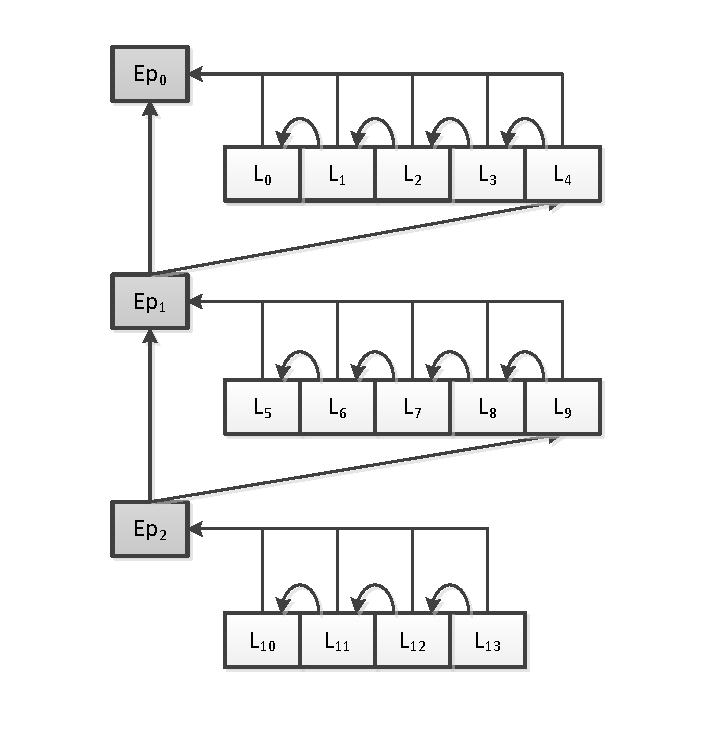
\includegraphics[scale=0.8]{images/hashchain.pdf} \\
%\caption{A visual depiction of the hash chain construction scheme. In this case, the epoch window is $5$ log entries, as shown by the epoch
%cycle after $5$ consecutive log entries.}
%\label{fig:hashChain}
%\end{figure*}

In this scheme the $X_i$ elements are used to link together consecutive entries in 
the hash chain. Similarly, the $Y_i$ elements are used to provide authentication 
for the $X_i$ element using an authentication tag for the $X_i$ entries. Also, the 
initial value for the MAC key $A_0$ is randomly generated when a user session is 
created. 

In order to prevent truncation and deletion attacks, a single entity $T_i$ for the entire log 
chain is updated as the log chain is iteratively constructed. Formally, $T_i$ is
computed as follows:
\begin{align*}
T_i = & HMAC_{B_i}(L_{i}, T_{i - 1}) \\
T_0 = & HMAC_{B_0}(L_{i}, 1)
\end{align*}
$B_0$ is a secret symmetrical key that that is randomly generated when the log chain for a user session
is initialized. This key is evolved with a pseudorandom function $H$ as follows:
\begin{align*}
B_{i+1} = H(B_i)
\end{align*}
For forward-security, this entity creation could be replaced with a publicly-verifiable Forward Secure Sequential Aggregate (FssAgg)
signature scheme backed by a trusted certificate authority to support forward-secure stream integrity. We refer the reader to 
\cite{Ma2008-FssAgg} for a more thorough treatment of FssAgg signature schemes and their role in updating the single log chain entity. 

%A visual representation of this protocol is shown in Figure \ref{fig:tagChain}. It is
%important to note that a chain of $T_i$ elements is not maintained. Instead, only the
%most recent element is persisted to the database. This is critical to prevent
%truncation attacks.

%\begin{figure*}[ht!]
%  \centering
%  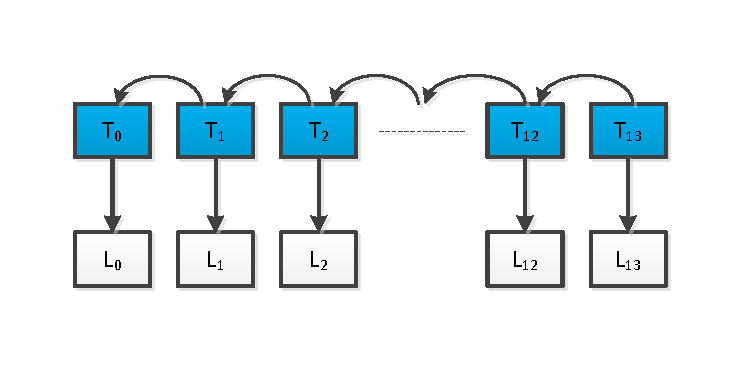
\includegraphics[scale=0.8]{images/tagchain.pdf} \\
%\caption{A visual depiction of the protocol used to build the log chain authentication tag.}
%\label{fig:tagChain}
%\end{figure*}

\subsection{Verification Modes}
\label{log:VerificationModes}

The ABLS log construction scheme enables two different modes of verification to be implemented,
each of which has different integrity and performance guarantees. The first mode of verification
requires one to walk the log chain, computing the digest $X_i$ and comparing it to the value
stored in the database. However, this method does not guarantee the integrity of the log chain.
The second mode of verification requires a trusted verifier task $\mathcal{V}$ to use the initial
hash chain key $A_0$ and entity key $B_0$ to walk the log entries, computing both $X_i$ and $Y_i$,
and comparing them against the values stored in the database. While this mode does not lend itself
to public verifiability, it guarantees the integrity of the log chain if a forward-secure MAC is used.

\section{Log Access Control}
Access control for log data is enforced using ciphertext policy attribute-based encryption 
(CP-ABE), a new encryption scheme that supports complex
access policies that specify which secret keys can be used for decryption \cite{Bethencourt2007-CPABE}. 
In CP-ABE, secret keys are analogous to sets of attributes, and access policies are defined using 
tree-like access structures of logical AND and OR gates, where each leaf in the tree is an attribute. Implementations of 
CP-ABE schemes are usually based on the construction of a bilinear mapping between two elliptic curve 
groups \cite{Bethencourt2007-CPABE} \cite{Junod2010-ABE}. We define both of these terms in the following sections.

\subsection{Mathematical Foundations}
\begin{definition}
Let $\mathbb{F}_p$ be a finite field where $p > 3$ is a prime, and $a, b \in \mathbb{F}_p$ such that
\begin{align*}
4a^3 + 27b^2 \not= 0 \mod p \in \mathbb{F}_p
\end{align*}

An \emph{ellptic curve} $E[\mathbb{F}_p]$ is the set of solutions $(x, y)$ to the equation
\begin{align*}
y^2 = x^3 + ax + b \mod p \in \mathbb{F}_p[x],
\end{align*}
together with the point at infinite $0$.
\end{definition}

\begin{definition}
Let $G_1$ and $G_2$ be cyclic groups of prime order $p$ and $g$ a generator of $G_1$. We say that $e$ is a \emph{bilinear map} defined as $e : G_1 \times G_2$, where $|G_1| = |G_2| = p$. This bilinear map satisfies the following properties:
\begin{itemize}
	\item Bilinearity: For all $u, v \in G_0$ and $a, b \in \mathbb{Z}_p$, we have $e(u^a, v^b) = e(u,v)^{ab}$
	\item Non-degeneracy: $e(g, g,) \not= 1$
	\item Computability: Both $G_1$ and $G_2$ are efficiently computable
\end{itemize}
\end{definition}

\subsection{Ciphertext Policy Attribute-Based Encryption}
In the original construction of the CP-ABE scheme, Bethencourt et al. \cite{Bethencourt2007-CPABE} defined five different procedures 
used in the cryptosystem: \emph{Setup}, \emph{Encrypt}, \emph{KeyGeneration}, \emph{Derypt}, and 
\emph{Delegate}. We define each of these procedures as follows:
\begin{itemize}
	\item \textbf{Setup} - This procedure takes the implicit security parameter as input and outputs the public and master keys $PK$ and $MK$.
	\item \textbf{Encrypt}(\textbf{PK}, M, $\mathbb{A}$) - This procedure will encrypt $M$, a plaintext message, to produce a ciphertext $CT$ such that only a user that possesses a set of attributes that satisfies the access structure $\mathbb{A}$ will be able to decrypt the message. The encryption process embeds $\mathbb{A}$ into the ciphertext.
	\item \textbf{KeyGeneration}(\textbf{MK}, $\mathbb{S}$) - This procedure generates a private key $SK$ using the master key $MK$ and set of attributes $S$ that describe the private key. 
	\item \textbf{Decrypt}(\textbf{PK}, \textbf{CT}, \textbf{SK}) - This procedure decrypts the ciphertext $CT$ using the provided secret key $SK$ to return the original message $M$. Decryption is only successful if the set $S$ of attributes, which is associated with the key $SK$, satisfies the access policy embedded within the ciphertext (which is part of the access structure $\mathbb{A}$).
	\item \textbf{Delegate}(\textbf{SK}, \~{S}) - This procedure outputs a secret key \~{$SK$} for the set of attributes \~{$S$}, where \~{$S$} $\subset S$, the set of attributes associated with the secret key \textbf{SK}.
\end{itemize}

\subsection{Access Policy Definition}

A major component of ABLS is the policy engine, which maps access policies defined on an event basis to 
the corresponding access tree used for encryption. For example, an access policy might state that only User
XYZ, or physician assistants or nurse practitioners from Medical Group A, are allowed to access data associated
with an event $E$. The corresponding access tree for this policy is shown in Figure \ref{fig:accessTree}.  

\begin{figure}[ht!]
\begin{center}
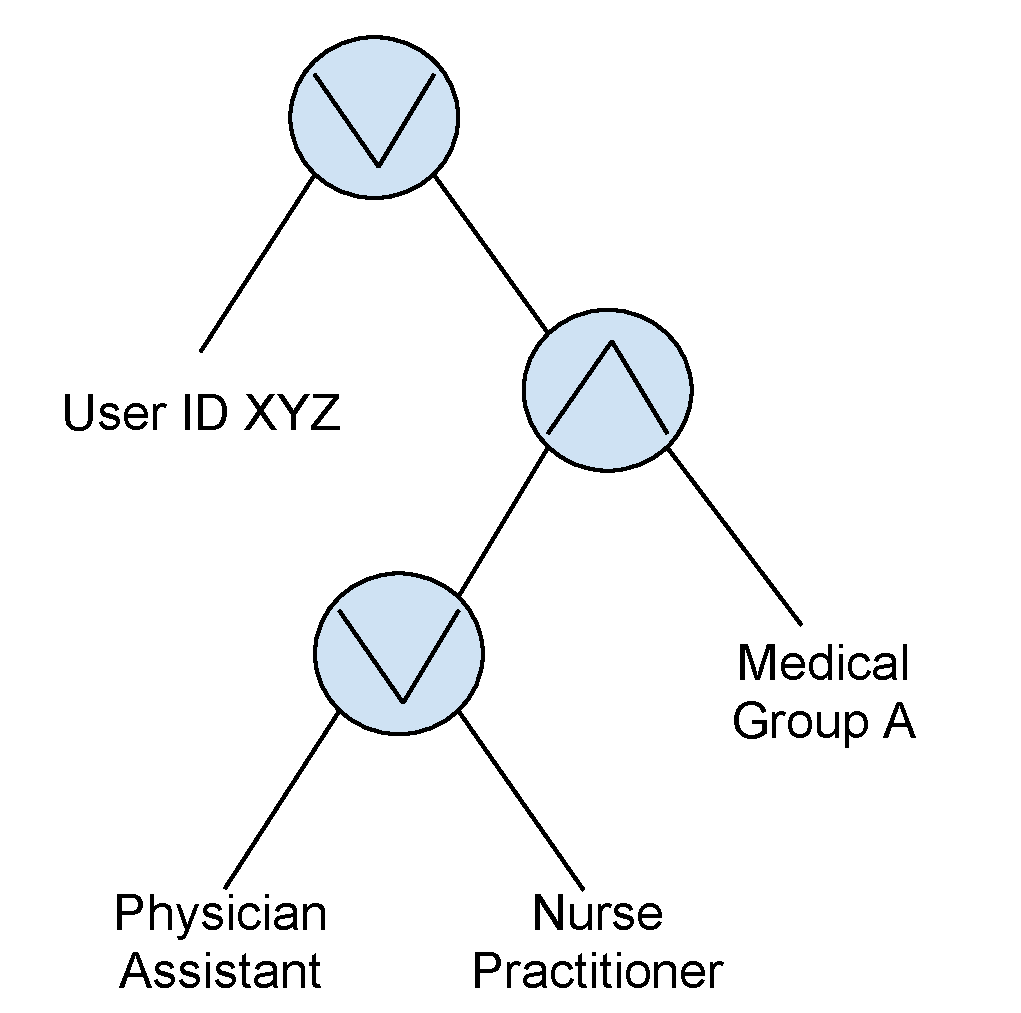
\includegraphics[width=1.5in]{images/cpabePolicy.pdf}
\caption{Access tree for a policy that only enables access to user XYZ, Medical Group A physician assistants, and Medical Group A nurse practitioners.}
\label{fig:accessTree}
\end{center}
\end{figure}

Our logging scheme makes the assumption that events, and the access policies for all data associated
with such events, are well defined, which is often the case with organizations that must
comply with federal legislation like HIPAA \cite{annas2003hipaa}. With this
assumption, the behavior of the policy engine in generating access policies is dependent on
administrator-defined policy rules for events of interest and the corresponding attributes of
system users and data that trigger such events. In this way, policy rules are coupled to events so that 
policies for access are generated based on the type of event that occurred and the user who is requesting 
access to such information. 

\begin{comment}
In this scheme, policy rules can be thought of as functions similar to the ones described by 
{\tt Rule-$E_1$} and {\tt Rule-$E_2$} (Algorithms \ref{alg:ruleE1} and \ref{alg:ruleE2}, respectively).

In this example, we see that the rule for event $E_1$ takes an {\tt EventInformation} structure, which contains
all of the information generated for an event. A prospective definition for an {\tt EventInformation} structure
is shown below.
\begin{lstlisting}
struct 
{
    User SourceUser;
    int EventId;
} 
EventInformation;
\end{lstlisting} 

The information contained within this structure is specific 
to the implementation of the system. For our purposes, we only require the source user from which the
event was generated, as well as the event identifier. The policy engine would then query the user
database to determine the secret identity of the source user and embed this in the resulting attribute
list. Optionally, depending on the implementation of {\tt RuleE1}, the policy engine would append additional
attributes to the list in disjunctive normal form. The simplicity of these policy implementations 
makes changing them an effortless task should the organization's security policy change.


\begin{algorithm}[ht] %[htb]
\caption{{\tt Rule-$E_1$} policy} \label{alg:ruleE1}
\begin{algorithmic}[1]
\REQUIRE{An {\tt EventInformation} object instance $e$.}
\ENSURE{The access policy for the event corresponding to the information in $e$}
\STATE{UserID $\leftarrow$ database.queryUserId(e.SourceUser)}
\STATE{Return ('UserID' OR 'Colleague of attributeID' OR 'System Administrator')}
\end{algorithmic}
\end{algorithm}

\begin{algorithm}[ht] %[htb]
\caption{{\tt Rule-$E_2$} policy} \label{alg:ruleE2}
\begin{algorithmic}[1]
\REQUIRE{An {\tt EventInformation} object instance $e$.}
\ENSURE{The access policy for the event corresponding to the information in $e$}
\STATE{UserID $\leftarrow$ database.queryUserId(e.SourceUser)}
\STATE{Return ('UserID' OR 'System Administrator')}
\end{algorithmic}
\end{algorithm}
\end{comment}

\subsection{Key Generation and Management}
Pairing-based cryptography is computationally expensive, and under the assumption that ABLS might be subject 
to very heavy traffic loads at any particular time, the 
overhead of encrypting data to be stored in the database should be as minimal as possible. Therefore, each unique
policy that is needed to encrypt a log message is associated with a symmetric key, which is in 
turn encrypted using CP-ABE and then serialized to be stored in the key database. 
This design enhancement enables increased throughput without sacrificing the 
level of confidentiality granularity that is needed for each log entry. However, should an 
unencrypted policy key for a given user's session become compromised, the remaining entries in that log database are at risk of being compromised. 

The basic procedure for encrypting a log entry is shown in Algorithm \ref{alg:encrypt}. Once encrypted, the ciphertext
is stored in the database with the rest of the information necessary to continue the log chain for a given user's session.
  
\begin{algorithm}[h] %[htb]
\caption{Log entry encryption} \label{alg:encrypt}
\begin{algorithmic}[1]
\REQUIRE{An unencrypted log entry $L_i$ for session $S_j$ of user $U_k$}
% \ENSURE{The number of all minimum $(s,t)$-cuts of $G$}

% I decided not to list the input/output in this case, so that's why the above two lines are commented out
\STATE{Let $P$ be the access control policy for the message of $L_i$, as determined by the {\tt PolicyEngine}}
\IF{The symmetric key $K$ for $(U_k, S_j)$ has not been generated for $P$}
  \STATE{Generate $K$ and encrypt it with the CP-ABE encryption module using $P$, yielding $K_E$}
  \STATE{Persist $K_E$ to the key database}
\ELSE
  \STATE{Query the database for $K_E$, the encrypted key for policy $P$.}
  \STATE{Decrypt $K_E$ using the attributes of user $U_k$, yielding $K$}
\ENDIF
\STATE{Encrypt $L_i$ with AES-256 using $K$, yielding $E(L_i, K)$}
\STATE{Persist $E(L_i, K)$ to the log database}
\end{algorithmic}
\end{algorithm}

In order to improve the performance of the logger, the per-policy symmetric keys used for encryption for a user session are kept
in memory until the session has been closed. This avoids the need for the logger to query the database for the key 
when a new log message arrives. 

By default, the secret keys used for decryption are never cached in the system's local memory. Since it is
expected that log entries will be read much less frequently than they will be written, such keys are generated
on demand by querying the appropriate database. Furthermore, the key generation process can be done in two ways. 
For policy rules that limit the access to only the generating user, only a single query to the attribute database
is required to establish the user's secret key and then decrypt the data for all log entries corresponding to that rule. 
With this key the user may decrypt these entries offline without the need to query the policy engine for the 
appropriate access rights.

Conversely, for access policy rules that embed attributes for colleagues or other users related to the 
source user, the policy engine must first query the user database to ensure the requesting 
user meets the relationship criteria set in place by the policy. Then,
if this is successful, the policy engine will grant the appropriate secret key to the requesting user. The tradeoff
is that, while an online TTP is needed for such colleagues to access the log entry contents, it is significantly easier
for the system administrators to manage who has access to specific log entries aside from the original source user.
Simply modifying the user's relationships in the system database is sufficient to revoke access from certain colleagues.

In order to maintain the security of the system at runtime, it is necessary to cycle the master and public keys
associated with the encryption scheme. Our current system does not support this feature, but there are two
ways that it could be implemented. The first way is to persist the old master and 
public keys to a safe location that could be called during auditing and verification if needed. The second way is 
to re-encrypt the entire log database with the new master and public key. Unfortunately, this would not only require the system to be 
brought offline during the update (in order to avoid synchronization issues with live traffic), but it would also
mean that the new master and public key serve as a single point of failure for the entire database if compromised. 
Therefore, future releases of this system plan to implement the first approach to manage keys. It would be
best to determine the key cycle lifetime based on empirical data associated with the growth of the log database.
Intuitively, in order to maintain auditing and verification efficiency, the cycle frequency should be defined as 
a monotonically increasing function that is proportional to the growth of the database. 

\section{Structured Log Data for Automated Audits}
Current technological solutions for automated audits in organizations where the usage of audit trails is required for compliance activities
are considered to be ineffective \cite{president2004revolutionizing}. In order to support automated audits of audit trails,
it is necessary to specify a formal structure for this data that matches organizational security policies. 
Therefore, a major motivating factor for the ABLS log data structure comes from realistic security policies. In this context, we make
the assumption that a security policy can be stated as a set of \emph{negative} requirements. For example, one 
such requirement might be that a doctor is not allowed to change their patient's address. In order to conduct an 
automated audit for violations of this policy, we first translate this semantically-rich requirement into a language
whose structure can be easily mapped to a relational data model. This enables us to leverage the power of 
structured query languages (i.e. SQL) to search for policy violations.

One solution for parsing security policy requirements into relational data is to define a grammar for producing 
requirement strings from a set of non-terminals that correspond to relations. Using the NIST RBAC model of
access control as motivation \cite{Ferraiolo2001-RBAC}, we specify this set of non-terminals and relations to 
be the set identifiers USER, OBS, OPS, and AFFECTEDUSERS. These finite sets are minimal enough to 
allow the specification of most security policies, thus making it suitable for our needs. 

LAudit, a simple context-free grammar that is built on these relations, is shown below.\\

{\setlength\tabcolsep{4pt}
\begin{tabular}{>{$}l<{$}>{$}r<{$}>{$}l<{$}}
  \text{LAudit} &\Coloneqq & \text{USER OPS}\\
  &| & \text{USER OPS OBS} \\
  &| & \text{USER OPS OBS USER} \\
\end{tabular}}
\vspace{.35cm} 

In this context, USER, OPS, and OBS are all finite sets composed of the users, operations, and objects of a
system, as specified by the NIST RBAC model \cite{Sandhu2000-nist-rbac}. While simple, this language effectively
captures the ``who'' and ``what'' of log events. ABLS is capable of appending a timestamp to every that it receives,
which rounds off the log event with ``when'' information. 

ABLS clients must submit log messages according to a pre-defined schema that captures
all of the information in LAudit. A JSON schema that can be used for constructing log messages 
is shown below.

\begin{lstlisting}
[
    {
        user : int,
        session : int,
        action : int (or String),
        object : int (or String),
        affectedUsers : [int]
    }
]
\end{lstlisting}

\section{Relational Model and Privacy Implications}
In order to capture the audit information in a relational model to enable efficient and automated queries, 
the events, actions, objects, and affected users are all coupled to the incoming log data. The resulting relational
model is shown in Figure \ref{fig:schema}.

This schema only corresponds to the log database in ABLS. There are in fact four databases altogether that must be maintained by ABLS:
the log, key, user, and policy database. The log database maintains all information in the log chain for every 
single user and session pair. The key database stores the cryptographic keys that were used to construct
such log chains. The user, and policy databases store user information and policy rules for ABLS, respectively. 

In order to link the entries in the log tables to their corresponding verification and encryption keys in the key database,
common user and session IDs are used (though not as the primary key for the tables since they do not satisfy
the uniqueness property). However, storing user and session information in plaintext may lead to a privacy violation
if the database is compromised. Therefore, using a technique similar to the ``onion encryption'' design in
CryptDB \cite{Popa2012-CryptDB}, this information is now deterministically encrypted before being stored in the database.

This procedure works by encrypting the user and session attributes with a symmetric key generated
from the logger's master key salted by the target table identifier. In mathematical
terms, the encrypted user and session IDs, $[U_i]$ and $[S_j]$, stored in table $T$ are generated as follows.
\begin{align*}
[U_i] = E(M_k || H(T), U_i) \\
[S_j] = E(M_k || H(T), S_j) \\
\end{align*}
In this context, $M_k$ is the master key for the logger. Using the table identifier as a salt to the master key 
enable ensures that tables do not share any common information about the user, which helps prevent against 
inference attacks in the event that the database servers are compromised. Furthermore, this enables verifiers,
who will have access to $M_k$ through the key manager, to decrypt log entries and recover the user identifier 
so that they may check the contents of the other databases as needed.

In the log data model, all Action and Object records are stored in plaintext. These tables store elements of a finite set, and
encrypting them would not derail a determined attacker. However, all information about affected users is encrypted 
(masked) using the aforementioned technique. As such, an attacker can infer
information about what types of objects were operated upon, but they cannot determine the specifics of these actions
or the users who performed them without compromising the ABLS master key $M_k$. We feel as though this strikes
a good balance between robust audit specification, reasonable measures of audit and log efficiency, user privacy, and log security. 

\begin{figure*}[htb!]
\begin{center}
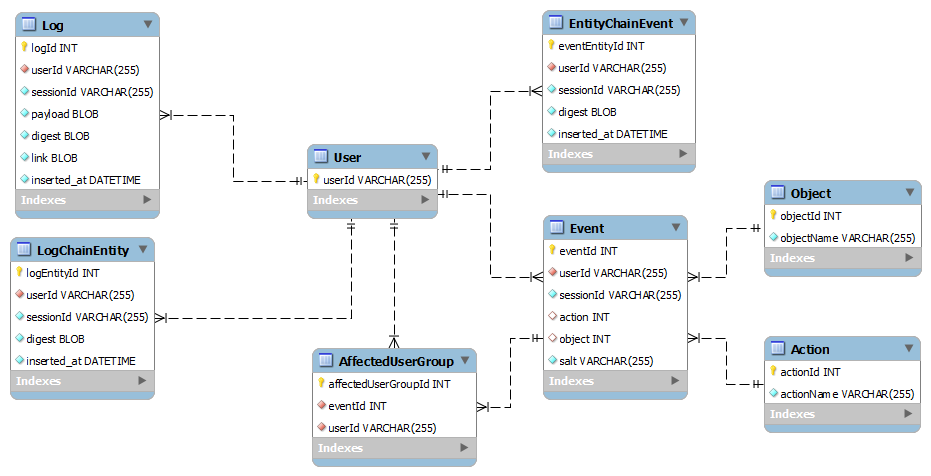
\includegraphics[width=5in]{images/logSchema.png}
\caption{ER diagram depicting the relational schema for the log data model.}
\label{fig:schema}
\end{center}
\end{figure*}

\section{Deployment}
\label{sec:deployment}
ABLS is designed to be a centralized logging system backed by a set of distributed databases. A context
diagram for the ABLS deployment scheme is shown in Figure \ref{fig:deployment}.

\begin{figure*}[htb!]
\begin{center}
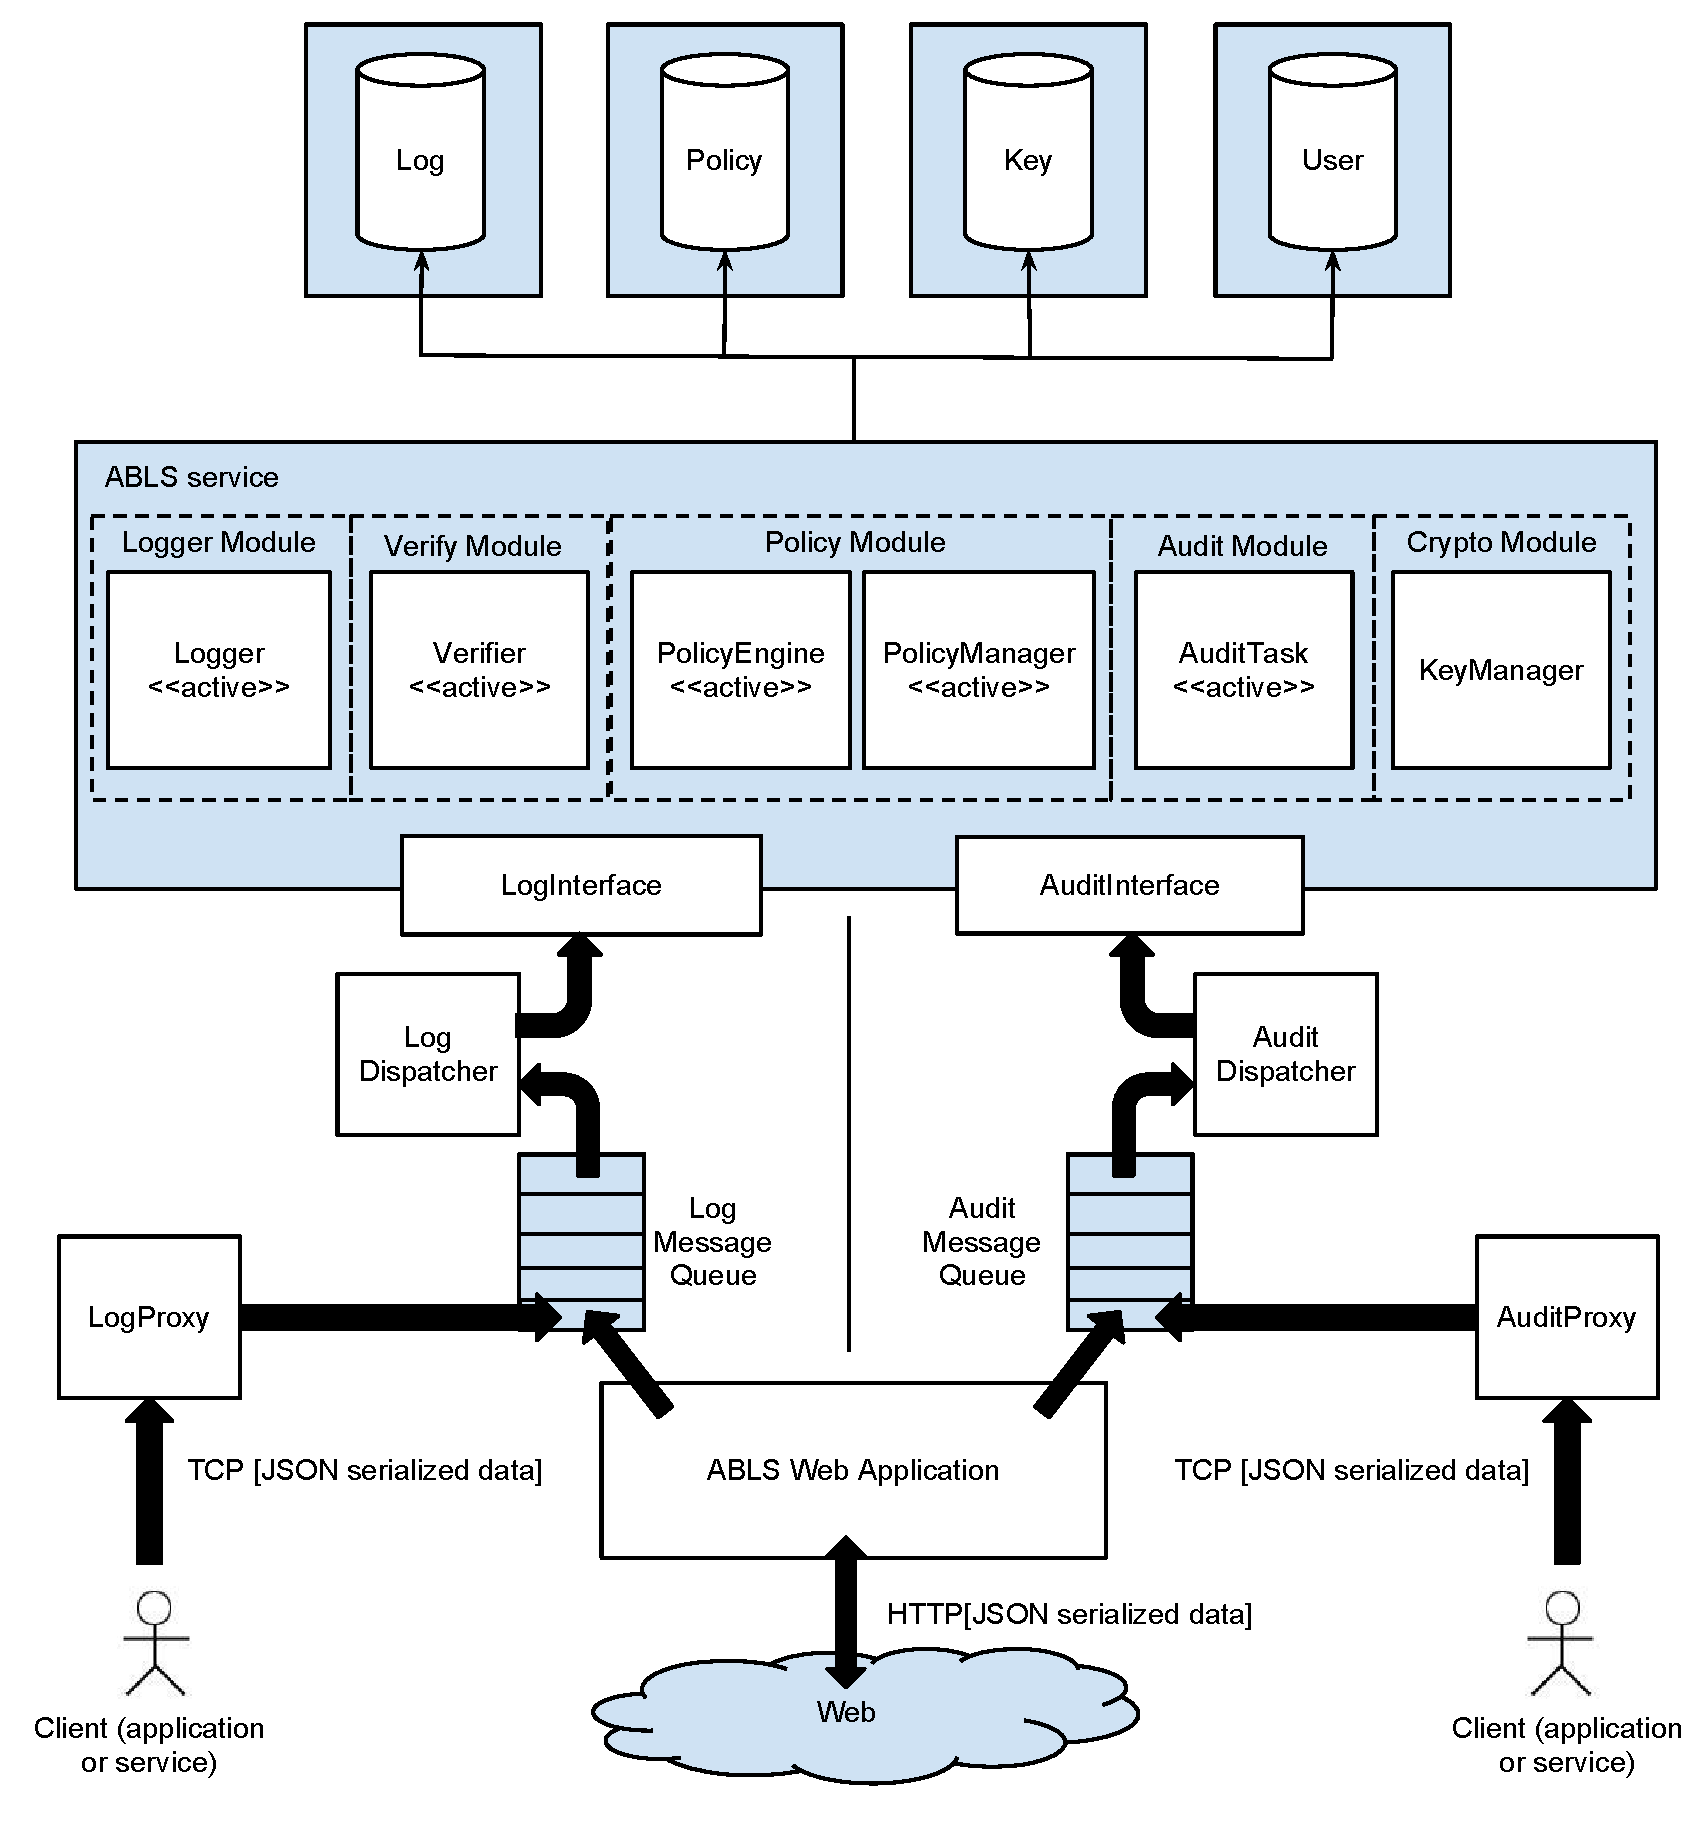
\includegraphics[width=5in]{images/deployment.pdf}
\caption{A high-level deployment diagram for ABLS.}
\label{fig:deployment}
\end{center}
\end{figure*}

Based on the purpose of each piece of data used in the log, it is best to physically separate databases
that store data of different security classes rather than rely on a single, segregated database that uses MAC with 
polyinstantiation to protect data of different security classes. Of course, access control
and authentication mechanisms for all of the database servers is to be enforced at the operating system level, thus
prohibiting immediate access to all unauthorized users other than the internal tasks (i.e. logger, verifier, policy engine, etc) 
within an ABLS instance. 

\section{Analysis}
The prototype ABLS system was written in Python, utilizing the Charm cryptography package 
\cite{akinyelecharm} for pairing-based cryptographic primitives. A major concern for this new architecture 
was its scalable performance while processing large amounts of log data. Therefore, we conducted experiments
to measure the encryption overhead from events that have uniform access policies, as well as the
encryption overhead from events that have different access policies. These two experiments were conducted to
guage the overhead of that results from log encryption and querying the policy engine for generating new policies.
The results for these two experiments are shown in Figures \ref{fig:logPerf} and \ref{fig:logPerfDiffEvents}.

\begin{figure}[ht!]
\begin{center}
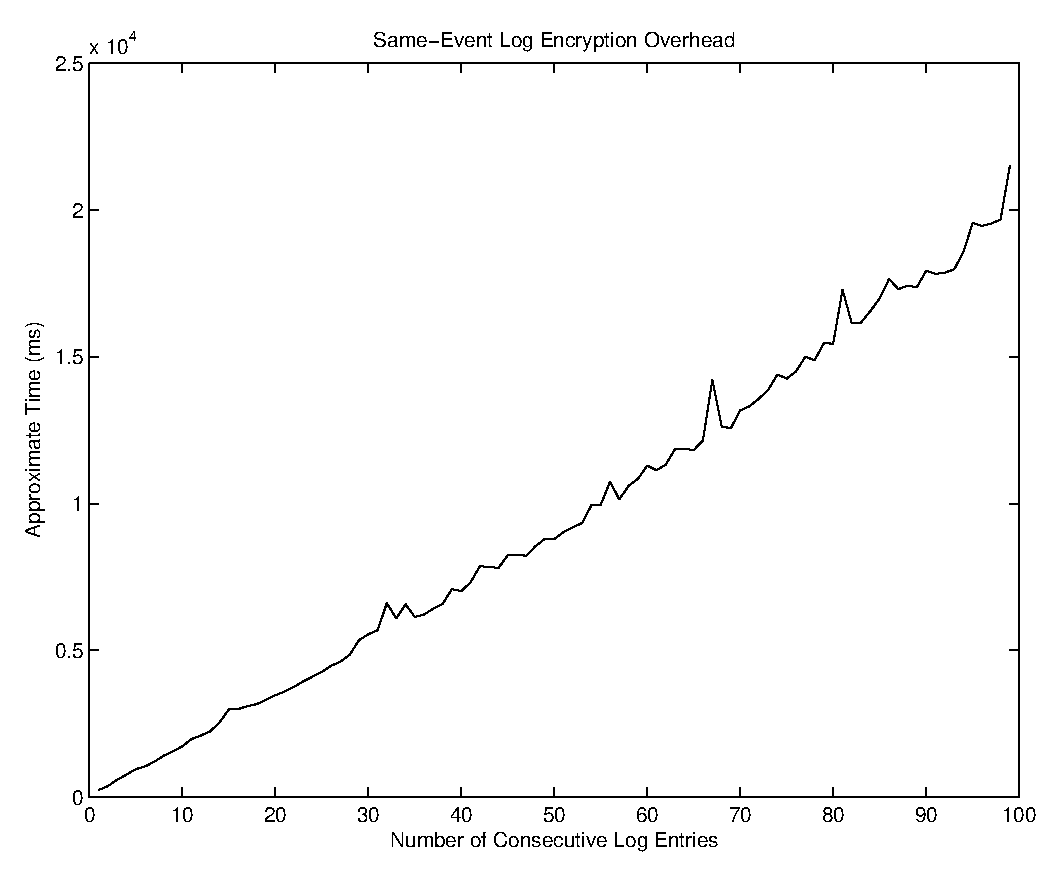
\includegraphics[width=3in]{images/logPerf.eps}
\caption{Log encryption performance for data in a single user session that all have the same access policy.}
\label{fig:logPerf}
\end{center}
\end{figure}

\begin{figure}[ht!]
\begin{center}
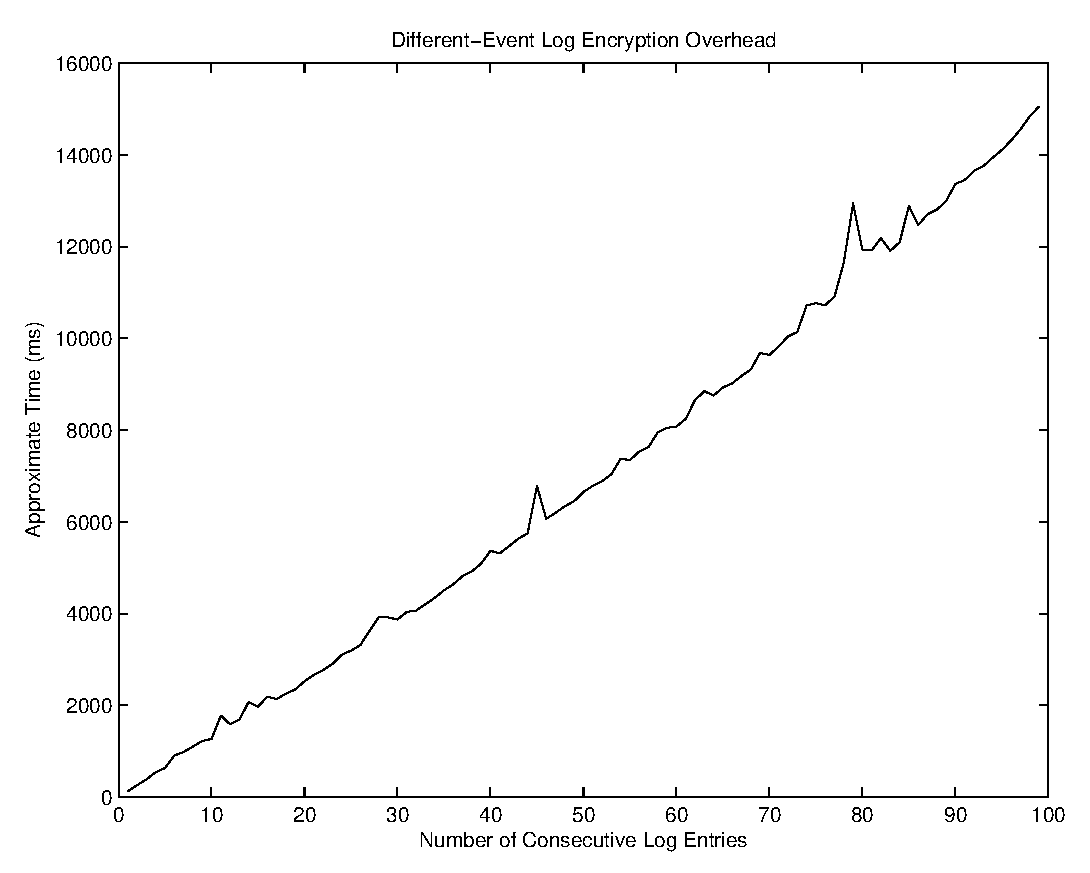
\includegraphics[width=3in]{images/logPerfDiffEvents.eps}
\caption{Log encryption performance for data in a single user session that all have different same access policies.}
\label{fig:logPerfDiffEvents}
\end{center}
\end{figure}

To measure the storage overhead for the log data we compared the physical size of an empty SQLite database against
one that contained log data for three different policies, each with different sets of attributes. The results of
this comparison are shown in Table \ref{tab:storage}. Based on this analysis, we concluded that each log entry contributed
approximately 1.2Kb of information to the log database, which is largely due to the highly conservative data types in the relational model.
This overhead could be drastically reduced if the model was adjusted to match the cryptographic primitives used in
the logging scheme and avoiding the use of BLOB attribute types.

\begin{table}
\label{tab:storage}
\caption{Storage overhead for storing the log data}
  \begin{tabular}{|l|l|}
    \hline
    Log Database Contents & Storage Size (Kb) \\ \hline
    None & 12 \\ 
    100 log entries - minimal attributes & 134 \\ 
    100 log entries - medium attributes & 147 \\ 
    100 log entries - maximum attributes & 149 \\
    \hline
  \end{tabular}
\end{table}

\section{Applications}
ABLS would be particularly useful in the healthcare domain, where organizations are required to comply with HIPAA policies
and regulations. Non-repudiation is a critical element that is needed to support these compliance efforts. Therefore,
configuring ABLS for use in these organizations can help securely collect and persist relevant log information, and 
also automate the auditing process to reinforce the manual efforts done by security administrators. In such an environment,
healthcare web applications would be configured to send all relevant user events to an ABLS instance in the cloud
via the HTTP API. All clients could be authenticated using a standard password-based scheme that is connected
the organization's user database.

Similarly, all dedicated health machines and terminals in hospitals and physician offices would maintain continuous 
data streams to an ABLS instance and send all log data over a TCP socket using an API similar to that which is exposed to
web applications. These dedicated entities could be authenticated using two-way SSL authentication so as to allow authentication
to take place using automatically exchanged SSL certificates.

Security administrators could review the organization's required security policies and encode them using the popular eXtensible
Access Control Markup Language (XACML), which could be used to configure the ABLS policy engine for encrypting all incoming log data.
Similarly, the security administrators could define automated audit tasks that ensure policy violations do not occur. The security
administrator would also be responsible for configuring the frequency at which automated audit and verification tasks and run. 
Although the current ABLS prototype does not currently export policy violations to a dashboard of any kind, in the event that 
this feature was added, the security administrator would also be responsible for configuring the connection between ABLS and the 
dashboard. Finally, depending on the rate at which the ABLS databases grow, the security administrator should also specify the 
parameters for archiving all audit data in a remote location. 

\section{Conclusion}
In this paper we presented ABLS, a secure logging system for the cloud that supports automated audits and dynamic,
attribute-based log file encryption. We discussed the log integrity and confidentiality properties supported by ABLS, 
and how they map to the underlying system architecture and relational data model. We then presented a sample deployment 
scheme for an ABLS instance in the cloud, which included the client interfaces for submitting log data and executing 
audit queries. We finished with a performance analysis of the current ABLS prototype and discussion of employing ABLS in 
the healthcare domain. This paper revealed that achieving automated audits is a non-trivial challenge that must strike
a balance between system performance and storage overhead. While the current ABLS design provides efficient automated
audits to help support non-repudiation, there are several fundamental design changes (i.e. the application of FssAgg 
signature generation algorithms to encrypted log chains) that can be explored for further improvement.

\begin{comment}
\begin{table}
\centering
\caption{Feelings about Issues}
\begin{tabular}{|l|r|l|} \hline
Flavor&Percentage&Comments\\ \hline
Issue 1 &  10\% & Loved it a lot\\ \hline
Issue 2 &  20\% & Disliked it immensely\\ \hline
Issue 3 &  30\% & Didn't care one bit\\ \hline
Issue 4 &  40\% & Duh?\\ \hline
\end{tabular}
\end{table}

\begin{figure}[htb]
\label{sample graphic}
\begin{center}
\includegraphics[width=1.5in]{fly.jpg}
\caption{A sample black \& white graphic (JPG).}
\end{center}
\end{figure}
\end{comment}

\bibliographystyle{abbrv}
\bibliography{../abls}
% You must have a proper ".bib" file
%  and remember to run:
% latex bibtex latex latex
% to resolve all references
\balance
\end{document}
